\documentclass[10pt,a4paper]{article}
\usepackage[latin1]{inputenc}
\usepackage[T1]{fontenc}
\usepackage{amsmath}
\usepackage{amsfonts}
\usepackage{amssymb}
\usepackage{graphicx}
\usepackage{hyperref}
\usepackage{amsthm}
\usepackage{tikz}
\usepackage{subcaption}
\usepackage{aligned-overset}
\usepackage[margin=2cm]{geometry}


\newtheorem{defn}{Definition}
\newtheorem{thm}{Theorem}


\author{Tobias Rohner}
\title{LehrFEM++ Hierarchic Finite Elements}


\begin{document}
    
\maketitle

\section{Polynomials}

    \begin{defn}
        Given $p \in \mathbb{N}$ and a polynomial $\psi(x) \in \mathcal{P}_p(\mathbb{R})$, we define the scaled polynomial $\psi(x;t)$ as
        \begin{equation*}
            \psi(x;t) := t^p\psi\left(\frac{x}{t}\right)
        \end{equation*}
    \end{defn}


\subsection{Shifted Legendre Polynomials}

    \begin{defn}[Shifted Legendre Polynomials]
        The Shifted Legendre Polynomials $P_n(\cdot;t) : [0, t] \to \mathbb{R}$ of degree $n \in \mathbb{N}$ are uniquely defined by the following properties:
        \begin{equation*}
            \int_0^1\! P_m(x;t)P_n(x;t) \,\mathrm{d}x = 0 \mbox{ if } m \neq n, \quad P_n(t;t) = 1
        \end{equation*}
    \end{defn}

    \begin{defn}[Integrated Shifted Legendre Polynomials]
        We define the Integrated Shifted Legendre Polynomials $L_n(\cdot;t) : [0, t] \to \mathbb{R}$ of degree $n \in \mathbb{N}$ as
        \begin{equation*}
            L_n(x;t) := \int_0^x\! P_{n-1}(\xi;t) \,\mathrm{d}\xi
        \end{equation*}
    \end{defn}

    We observe that due to the orthogonality condition of the Legendre Polynomials, the Integrated Legendre Polynomials of order $n \geq 2$ are zero at $x \in \{0, t\}$:
    \begin{align*}
        L_n(0;t) &= \int_0^0\! P_{n-1}(\xi;t) \,\mathrm{d}\xi = 0 \\
        L_n(t;t) &= \int_0^t\! P_{n-1}(\xi;t) \,\mathrm{d}\xi = \int_0^t\! P_{n-1}(\xi;t)P_0(\xi;t) \,\mathrm{d}\xi = 0, \mbox{ for } n \geq 2
    \end{align*}
    
%    \begin{thm}
%        A recurrence relation for the \textit{Shifted Legendre Polynomials} $P_n(x;t) : [0,t] \to \mathbb{R}$ is given by
%        \begin{align*}
%            P_0(x;t) &= 1 \\
%            P_1(x;t) &= 2x - t \\
%            nP_n(x;t) &= (2n-1)(2x-t)P_{n-1}(x;t) - (n-1)t^2P_{n-2}(x;t) \mbox{ for } n \geq 2
%        \end{align*}
%    \end{thm}
%
%    \begin{thm}
%        A recurrence relation for the derivative of the \textit{Scaled Shifted Legendre Polynomials} $\partial_x P_n(x;t) : [0,t] \to \mathbb{R}$ is given by
%        \begin{align*}
%            \partial_x P_0(x;t) &= 0 \\
%            \partial_x P_n(x;t) &= 2nP_{n-1}(x;t) + (2x-t)\partial_xP_{n-1}(x;t) \mbox{ for } n \geq 1
%        \end{align*}
%    \end{thm}
%
%    \begin{thm}
%        A recurrence relation for the \textit{Integrated Shifted Legendre Polynomials} $L_n(\cdot;t) : [0, t] \to \mathbb{R}$ is given by
%        \begin{align*}
%            L_1(x;t) &= x \\
%            2(2n-1)L_n(x;t) &= P_n(x;t) - t^2P_{n-2}(x;t) \mbox{ for } n \geq 2
%        \end{align*}
%    \end{thm}
%
%    \begin{thm}
%        The derivative w.r.t. $x$ of the Integrated Shifted Legendre Polynomials is given by
%        \begin{equation*}
%            \partial_x L_n(x;t) = P_{n-1}(x;t)
%        \end{equation*}
%    \end{thm}
%
%    \begin{thm}
%        A recurrence relation of the derivative w.r.t. $t$ of the Integrated Shifted Legendre Polynomials is given by
%        \begin{align*}
%            \partial_t L_1(x;t) &= 0 \\
%            \partial_t L_n(x;t) &= -\frac{1}{2} \left( P_{n-1}(x;t) + tP_{n-2}(x;t) \right) \mbox{ for } n \geq 2
%        \end{align*}
%    \end{thm}
    
    
\subsection{Jacobi Polynomials}

    \begin{defn}[Jacobi Polynomials]
        The Jacobi Polynomials $\tilde{P}_n^{(\alpha,\beta)} : [-1, 1] \to \mathbb{R}$ of degree $n \in \mathbb{N}$ are uniquely defined by the following properties:
        \begin{equation*}
            \int_{-1}^1\! (1-x)^{\alpha}(1+x)^{\beta}\tilde{P}_n^{(\alpha,\beta)}(x)\tilde{P}_m^{(\alpha.\beta)}(x) \,\mathrm{d}x, \quad \tilde{P}_n^{(\alpha,\beta)}(1) = \binom{n+\alpha}{n}
        \end{equation*}
    \end{defn}

    \begin{defn}[Shifted Legendre Polynomials]
        We define the Shifted Legendre Polynomials $P_n^{(\alpha,\beta)} : [0, 1] \to \mathbb{R}$ of degree $n \in \mathbb{N}$ as
        \begin{equation*}
            P_n^{(\alpha,\beta)}(x) := \tilde{P}_n^{(\alpha,\beta)}(2x-1)
        \end{equation*}
    \end{defn}

    \begin{defn}[Integrated Shifted Legendre Polynomials]
        We define the Integrated Shifted Legendre Polynomials $L_n^{(\alpha,\beta)} : [0, 1] \to \mathbb{R}$ of degree $n \in \mathbb{N}$ as
        \begin{equation*}
            L_n^{(\alpha,\beta)}(x) := \int_0^x\! P_{n-1}^{(\alpha,\beta)}(x) \,\mathrm{d}x
        \end{equation*}
    \end{defn}

    For the sake of notational simplicity, we allow ourselves to ignore writing the $\beta$ parameter if it is equal to zero. We therefore have that
    \begin{equation*}
        P_n^{\alpha}(x) := P_n^{(\alpha,0)}(x), \quad L_n^{\alpha}(x) := L_n^{(\alpha,0)}(x)
    \end{equation*}


\section{Orientation Problems}

    \begin{figure}[ht!]
        \center
        \begin{subfigure}{0.45\textwidth}
            \center
            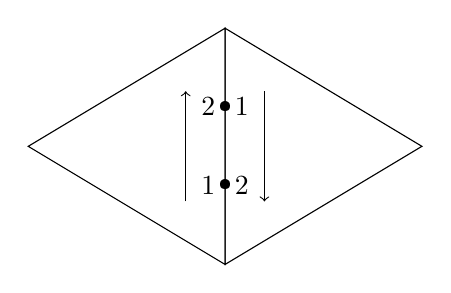
\begin{tikzpicture}
                % Draw the two triangles
                \draw[] (-2.5,0) -- (0,1.5) -- (0,-1.5) -- cycle;
                \draw[] (2.5,0) -- (0,-1.5) -- (0,1.5) -- cycle;
                % The orientation of the shared edge
                \draw[->] (-0.5,-0.7) -- (-0.5,0.7);
                \draw[->] (0.5,0.7) -- (0.5,-0.7);
                % Draw the conflicting DOF nodes on the shared edge
                \node at (0,0.5) {\textbullet};
                \node[anchor=west] at(0,0.5) {1};
                \node[anchor=east] at(0,0.5) {2};
                \node at (0,-0.5) {\textbullet};
                \node[anchor=west] at(0,-0.5) {2};
                \node[anchor=east] at(0,-0.5) {1};
            \end{tikzpicture}
        \end{subfigure}
        \begin{subfigure}{0.45\textwidth}
            \center
            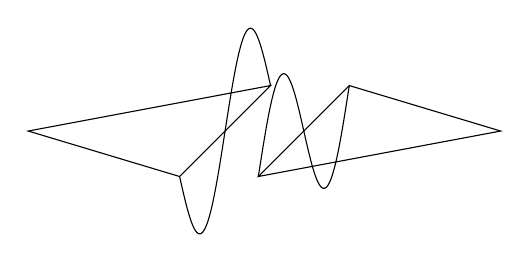
\begin{tikzpicture}
                % Draw the two triangles
                \draw[] (-3,0,0) -- (-0.5,0,1.5) -- (-0.5,0,-1.5) -- cycle;
                \draw[] (3,0,0) -- (0.5,0,-1.5) -- (0.5,0,1.5) -- cycle;
                % Draw the mismatched basis functions
                \draw[] (-0.5,0,-1.5)
                    \foreach \x in {1,...,100} {
                        -- (-0.5,{sin(3.6*\x)},{3*(\x-50)/100})
                    };
                \draw[] (0.5,0,-1.5)
                    \foreach \x in {1,...,100} {
                        -- (0.5,{sin(-3.6*\x)},{3*(\x-50)/100})
                    };
            \end{tikzpicture}
        \end{subfigure}
        \caption{Orientation Problem with Non-Lagrangian Finite Elements}
        \label{fig:orientation_problem}
    \end{figure}

    When using Lagrangian Finite Elements, we rely on the so called "glueing" in order to have a function space containing only continuous functions. This continuity is achieved by having a local numbering of DOFs as illustrated in \autoref{fig:orientation_problem} on the left. A single DOF may have different indices in the neighboring cells. Because the DOFs are symmetrically distributed on the edge, the two local basis functions of the neighboring cells will conveniently be continuous along the shared edge. However, if we do not use Lagrangian FEM, as is the case for Hierarchical FEM where the $n$-th edge DOF is the basis function coefficient for a polynomial of degree $n$, we no longer have continuity along the mesh edges (\autoref{fig:orientation_problem} on the right). In order to fix this, we must introduce a global ordering of the edge DOFs, as well as a global orientation of the edges. This is not a big problem though, as LehrFem++ mesh entities provide a function to access the global orientation of their edges. In the case the local orientation is flipped, we simply also flip the order of the local DOFs and the local coordinates at which we evaluate the edge basis functions. In the following sections, we will ignore this ordering problem and one simply has to apply the aforementioned transformations in order to obtain the basis on an arbitrary mesh entity.


\section{Basis Functions}

    We differentiate between three types of basis functions. The vertex basis functions, the edge basis functions and the face bubbles. The vertex basis functions will be nonzero on exactly one vertex and zero on all the others. The edge basis functions will be nonzero on an edge and zero on all other edges and the vertices. The face bubbles are nonzero only on the interior of the mesh entity while being zero on its boundary.


\subsection{Segment}

    \begin{figure}[ht!]
        \center
        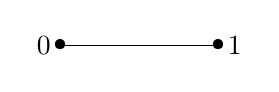
\begin{tikzpicture}
            % Edges
            \draw[] (0,0) -- (2,0);
            % Vertices
            \node at (0,0) {\textbullet};
            \node[anchor=east] at (0,0) {0};
            \node at (2,0) {\textbullet};
            \node[anchor=west] at (2,0) {1};
        \end{tikzpicture}
        \caption{Reference Element for the Segment}
        \label{fig:ref_segment}
    \end{figure}
    
    \begin{defn}[Vertex Basis Functions]
        We define the vertex basis functions on the reference segment as
        \begin{align*}
            \widehat{b_0^{\cdot}}(x) &:= 1 - x \\
            \widehat{b_1^{\cdot}}(x) &:= x
        \end{align*}
    \end{defn}

    \begin{defn}[Edge Basis Functions]
        We define the edge basis functions on the reference segment as
        \begin{equation*}
            \widehat{b_n^{-}}(x) := L_n(x) \mbox{ for } n \geq 2
        \end{equation*}
    \end{defn}


\subsection{Quadrilateral}

    \begin{figure}[ht!]
        \center
        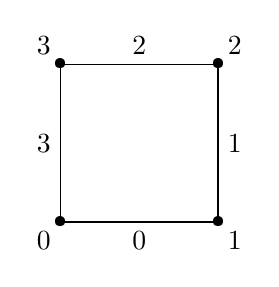
\begin{tikzpicture}
            % Edges
            \draw[] (0,0) -- (2,0) -- (2,2) -- (0,2) -- cycle;
            \node[anchor=north] at (1,0) {0};
            \node[anchor=west] at (2,1) {1};
            \node[anchor=south] at (1,2) {2};
            \node[anchor=east] at (0,1) {3};
            % Vertices
            \node at (0,0) {\textbullet};
            \node[anchor=north east] at (0,0) {0};
            \node at (2,0) {\textbullet};
            \node[anchor=north west] at (2,0) {1};
            \node at (2,2) {\textbullet};
            \node[anchor=south west] at (2,2) {2};
            \node at (0,2) {\textbullet};
            \node[anchor=south east] at (0,2) {3};
        \end{tikzpicture}
        \caption{Reference Element for the Quadrilateral}
        \label{fig:ref_quad}
    \end{figure}

    Each basis function on the quadrilateral is given by the product of two 1D basis functions of the segment. We obtain the following set of basis functions.
    
    \begin{defn}[Vertex Basis Functions]
        We define the vertex basis functions on the reference quadrilateral as
        \begin{align*}
            \widehat{b_0^{\cdot}}(x,y) &:= (1-x)(1-y) \\
            \widehat{b_1^{\cdot}}(x,y) &:= x(1-y) \\
            \widehat{b_2^{\cdot}}(x,y) &:= xy \\
            \widehat{b_3^{\cdot}}(x,y) &:= (1-x)y
        \end{align*}
    \end{defn}

    \begin{defn}[Edge Basis Functions]
        We define the edge basis functions $\widehat{b_{e,n}^{-}}(x,y)$ where $e \in \{0,1,2,3\}$ is the index of the edge and $n \geq 2$ the degree of the basis function as
        \begin{align*}
            \widehat{b_{0,n}^{-}}(x,y) &:= (1-y)L_n(x) \\
            \widehat{b_{1,n}^{-}}(x,y) &:= xL_n(y) \\
            \widehat{b_{2,n}^{-}}(x,y) &:= yL_n(x) \\
            \widehat{b_{3,n}^{-}}(x,y) &:= (1-x)L_n(y)
        \end{align*}
    \end{defn}

    \begin{defn}[Face Bubbles]
        We define the face bubbles on the reference quadrilateral as
        \begin{equation*}
            \widehat{b_{n,m}^{\square}}(x,y) := L_n(x)L_m(y)
        \end{equation*}
        where $n \geq 2$, $m\geq 2$.
    \end{defn}


\subsection{Triangle}

    \begin{figure}[ht!]
        \center
        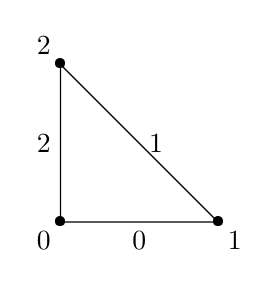
\begin{tikzpicture}
            % Edges
            \draw[] (0,0) -- (2,0) -- (0,2) -- cycle;
            \node[anchor=north] at (1,0) {0};
            \node[anchor=west] at (1,1) {1};
            \node[anchor=east] at (0,1) {2};
            % Vertices
            \node at (0,0) {\textbullet};
            \node[anchor=north east] at (0,0) {0};
            \node at (2,0) {\textbullet};
            \node[anchor=north west] at (2,0) {1};
            \node at (0,2) {\textbullet};
            \node[anchor=south east] at (0,2) {2};
        \end{tikzpicture}
        \caption{Reference Element for the Triangle}
        \label{fig:ref_tria}
    \end{figure}

    For the ease of notation, we make use of the Barycentric Coordinates given by
    \begin{equation*}
        \lambda_0 = 1-x-y,\quad \lambda_1 = x,\quad \lambda_2 = y.
    \end{equation*}
    
    \begin{defn}[Vertex Basis Functions]
        We define the vertex basis functions on the reference triangle as
        \begin{align*}
            \widehat{b_0^{\cdot}}(x,y) &:= \lambda_0 \\
            \widehat{b_1^{\cdot}}(x,y) &:= \lambda_1 \\
            \widehat{b_2^{\cdot}}(x,y) &:= \lambda_2 \\
        \end{align*}
    \end{defn}

    \begin{defn}[Edge Basis Functions]
        We define the edge basis functions $\widehat{b_{e,n}^{-}}(x,y)$ where $e \in \{0,1,2\}$ is the index of the edge and $n \geq 2$ the degree of the basis function as
        \begin{align*}
            \widehat{b_{0,n}^{-}}(x,y) &:= L_n(\lambda_1 ; \lambda_0+\lambda_1) \\
            \widehat{b_{1,n}^{-}}(x,y) &:= L_n(\lambda_2 ; \lambda_1+\lambda_2) \\
            \widehat{b_{2,n}^{-}}(x,y) &:= L_n(\lambda_0 ; \lambda_2+\lambda_0) \\
        \end{align*}
        Note that due to the scaling, the basis functions are only nonzero on the edge they are associated with. Furthermore, they are zero on all vertices.
    \end{defn}

    \begin{defn}[Face Bubbles]
        We define the face bubbles on the reference triangle as the product of an edge basis function with a blending polynomial.
        \begin{equation*}
            \widehat{b_{n,m}^{\triangle}}(x,y) := L_m^{2n}(\lambda_2)L_n(\lambda_1 ; \lambda_0+\lambda_1)
        \end{equation*}
        where $n \geq 2$, $m \geq 1$ and $n+m \leq q+1$ where $q$ is the interior degree of the basis functions.
    \end{defn}


\section{Dual Basis}

    The dual basis is used to find the basis function coefficients from a set of function evaluations at a predefined set of locations. This must be implemented this way, as a simple matrix inversion to solve for the coefficients is not stable enough for higher polynomial degrees.
    
    We again differentiate between the dual basis associated with the vertices, the edges, and the interior of a cell. It is important to notice that the dual bases must be orthogonalized with respect to the dual bases on the lower dimensional subentities. This is done using Gram-Schmidt and is omitted in the following.


\subsection{Segment}

    \begin{thm}[Vertex Dual Basis]
        The vertex dual basis on the reference segment is given by
        \begin{align*}
            \lambda_0^{\cdot}[f] &= f(0) \\
            \lambda_1^{\cdot}[f] &= f(1)
        \end{align*}
    \end{thm}
    \begin{proof}
        We plug the vertex basis functions into the dual basis to obtain
        \begin{align*}
            &\lambda_0^{\cdot}[\widehat{b_0^{\cdot}}] = \widehat{b_0^{\cdot}}(0) = 1, &\lambda_0^{\cdot}[\widehat{b_1^{\cdot}}] = \widehat{b_1^{\cdot}}(0) = 0 \\
            &\lambda_1^{\cdot}[\widehat{b_0^{\cdot}}] = \widehat{b_0^{\cdot}}(0) = 0, &\lambda_1^{\cdot}[\widehat{b_1^{\cdot}}] = \widehat{b_1^{\cdot}}(0) = 1
        \end{align*}
    \end{proof}

    \begin{thm}[Edge Dual Basis]
        The edge dual basis on the reference segment is given by
        \begin{equation*}
            \lambda_n^{-}[f] = (2n-1) \left( P_{n-1}(1)f(1) - P_{n-1}(0)f(0) - \int_0^1\! P_{n-1}'(x)f(x) \,\mathrm{d}x \right)
        \end{equation*}
    \end{thm}
    \begin{proof}
        Plugging in the edge basis functions gives
        \begin{align*}
            \frac{1}{2n-1}\lambda_n^{-}[\widehat{b_m^{-}}] &= \frac{1}{2n-1}\lambda_n^{-}[L_m] = P_{n-1}(1)L_m(1) - P_{n-1}(0)L_m(0) - \int_0^1\! P_{n-1}'(x)L_m(x) \,\mathrm{d}x \\
            &= \int_0^1\! P_{n-1}(x)L_m'(x) \,\mathrm{d}x = \int_0^1\! P_{n-1}(x)P_{m-1}(x) \,\mathrm{d}x = \frac{1}{2n-1}\delta_{n,m}
        \end{align*}
    \end{proof}

    Note that for the edge dual basis there is no need to orthogonalize with respect to the vertex basis functions because of the orthogonality of the Legendre polynomials.


\subsection{Quadrilateral}

    All basis functions on the quadrilateral are the tensor product of two basis functions on the segment. We can therefore reuse the segment dual basis to construct a dual basis for the quadrilateral.
    
    \begin{thm}
        Let $f : [0,1]^2 \to \mathbb{R}$ be a function to which we want to apply the dual basis. We define the function $f_y : [0,1] \to \mathbb{R}$ indexed by $y \in [0,1]$ to be $x \mapsto f(x, y)$. Applying the dual basis on the segment to this function, we are left with $g : [0,1] \to \mathbb{R}$ given by $g(y) = \lambda_n[f_y]$. We finally apply the dual basis of the segment to this function $g$ to obtain the result of applying the quadrilateral dual basis to $f$.
    \end{thm}
    \begin{proof}
        Let $\widehat{b^{\square}} : [0,1]^2 \to \mathbb{R}$ be an arbitrary basis function on the quadrilateral. As the quadrilateral basis is the tensor product of the basis on the segment, the function is separable into two basis functions on the segment $\widehat{b_i^{-}}$ and $\widehat{b_j^{-}}$ such that $\widehat{b^{\square}}(x,y) = \widehat{b_i^{-}}(x)\widehat{b_j^{-}}(y)$. We then have that
        \begin{equation*}
            g(y) = \lambda_m[f_y] = \lambda_m[\widehat{b_i^{-}}(x)\widehat{b_j^{-}}(y)] = \widehat{b_i^{-}}(x)\lambda_m[\widehat{b_j^{-}}(y)] = \widehat{b_i^{-}}(x)\delta_{j,m}
        \end{equation*}
        where $\lambda_n[\cdot]$ is an element of the dual basis of the segment. Finally applying the dual basis of the segment to the resulting $g(y)$, we see that
        \begin{equation*}
            \lambda_n[g(y)] = \lambda_n[\widehat{b_i^{-}}(x)\delta_{j,m}] = \lambda_n[\widehat{b_i^{-}}(x)]\delta_{j,m} = \delta_{i,n}\delta_{j,m}
        \end{equation*}
        proving that the given procedure yields a dual basis on the quadrilateral.
    \end{proof}

    For the same reason as in the case of the segment, we do not need to orthogonalize the resulting dual basis for the quadrilateral.


\subsection{Triangle}

    \begin{thm}[Vertex Dual Basis]
        The vertex dual basis on the reference triangle is given by
        \begin{align*}
            \lambda_0^{\cdot}[f] &= f(0,0) \\
            \lambda_1^{\cdot}[f] &= f(1,0) \\
            \lambda_2^{\cdot}[f] &= f(0,1)
        \end{align*}
    \end{thm}
    \begin{proof}
        We simply plug the vertex basis functions into the dual basis to obtain
        \begin{align*}
            \lambda_0^{\cdot}[\widehat{b_0^{\cdot}}] = \widehat{b_0^{\cdot}}(0,0) = 1,\quad \lambda_0^{\cdot}[\widehat{b_1^{\cdot}}] = \widehat{b_1^{\cdot}}(0,0) = 0,\quad \lambda_0^{\cdot}[\widehat{b_2^{\cdot}}] = \widehat{b_2^{\cdot}}(0,0) = 0 \\
            \lambda_1^{\cdot}[\widehat{b_0^{\cdot}}] = \widehat{b_0^{\cdot}}(1,0) = 0,\quad \lambda_1^{\cdot}[\widehat{b_1^{\cdot}}] = \widehat{b_1^{\cdot}}(1,0) = 1,\quad \lambda_1^{\cdot}[\widehat{b_2^{\cdot}}] = \widehat{b_2^{\cdot}}(1,0) = 0 \\
            \lambda_2^{\cdot}[\widehat{b_0^{\cdot}}] = \widehat{b_0^{\cdot}}(0,1) = 0,\quad \lambda_2^{\cdot}[\widehat{b_1^{\cdot}}] = \widehat{b_1^{\cdot}}(0,1) = 0,\quad \lambda_2^{\cdot}[\widehat{b_2^{\cdot}}] = \widehat{b_2^{\cdot}}(0,1) = 1
        \end{align*}
    \end{proof}

    \begin{thm}[Edge Dual Basis]
        The edge dual basis $\lambda_{e,n}[\cdot]$ on the reference triangle where $e \in \{0,1,2\}$ is the index of the edge is given by the segment dual basis applied along the edge. It is given by
        \begin{align*}
            \lambda_{0,n}^{-}[f] &= (2n-1)\left( P_{n-1}(1)f(1,0) - P_{n-1}(0)f(0,0) - \int_0^1\! p_{n-1}'(x)f(x,0) \,\mathrm{d}x \right) \\
            \lambda_{1,n}^{-}[f] &= (2n-1)\left( P_{n-1}(1)f(0,1) - P_{n-1}(0)f(1,0) - \int_0^1\! p_{n-1}'(x)f(1-x,x) \,\mathrm{d}x \right) \\
            \lambda_{2,n}^{-}[f] &= (2n-1)\left( P_{n-1}(1)f(0,1) - P_{n-1}(0)f(0,0) - \int_0^1\! p_{n-1}'(x)f(0,1-x) \,\mathrm{d}x \right)
        \end{align*}
    \end{thm}
    \begin{proof}
        We observe that the triangle basis functions parametrized along an edge reduce to the segment basis functions.
        \begin{align*}
            \widehat{b_{0,n}^{-}}(x,0) &= L_n(x;(1-x)+x) L_n(x;1) = L_n(x) \\
            \widehat{b_{1,n}^{-}}(1-x,x) &= L_n(x;(1-x)+x) = L_n(x;1) = L_n(x) \\
            \widehat{b_{2,n}^{-}}(0,1-x) &= L_n(1-(1-x);(1-x)+(1-(1-x))) = L_n(x;1) = L_n(x).
        \end{align*}
        Therefore, the proof is reduced to the proof for the dual basis of the segment.
    \end{proof}

    \begin{thm}[Face Dual Basis]
        The dual basis for the face bubbles on the reference triangle is given by
        \begin{equation*}
            \lambda_{n,m}^{\triangle}[f] = (2n-1)(2n+2m-1)\left( \int_0^1\!\int_0^{1-y}\! f(x,y)\left((1-y)^{i-1}{L_m^{2n}}''(y)-2n(1-y)^{n-2}{L_m^{2n}}'(y)\right)L_n''\left(\frac{x}{1-y}\right) \,\mathrm{d}x\mathrm{d}y \right)
        \end{equation*}
        for $n \geq 2$, $m \geq 1$ and $n+m \leq q+1$ where $q$ is the degree of the basis functions.
    \end{thm}
    \begin{proof}
        Plugging in the face bubbles while ignoring the normalization factor $(2n-1)(2n+2m-1)$ gives
        \begin{align*}
            \lambda_{n,m}^{\triangle}[\widehat{b_{i,j}^{\triangle}}] &= \int_0^1\!\int_0^{1-y}\! L_j^{2i}(y)L_i(x;1-y)\left((1-y)^{n-1}{L_m^{2n}}''(y)-2n(1-y)^{n-2}{L_m^{2n}}'(y)\right)L_n''\left(\frac{x}{1-y}\right) \,\mathrm{d}x\mathrm{d}y \\
            &= \int_0^1\!\int_0^{1-y}\! L_j^{2i}(y)L_i\left(\frac{x}{1-y}\right)\left((1-y)^{2n-1}{L_m^{2n}}''(y)-2n(1-y)^{2n-2}{L_m^{2n}}'(y)\right)L_n''\left(\frac{x}{1-y}\right) \,\mathrm{d}x\mathrm{d}y \\
            \overset{z=\frac{x}{1-y}}&{=} \int_0^1\!\int_0^1\! L_j^{2i}(y)L_i(z)\left((1-y)^{2n}{L_m^{2n}}''(y)-2n(1-y)^{2n-1}{L_m^{2n}}'(y)\right)L_n''(z)) \,\mathrm{d}z\mathrm{d}y \\
            &= \underbrace{\left( \int_0^1\! L_j^{2i}(y)\left((1-y)^{2n}{L_m^{2n}}''(y)-2n(1-y)^{2n-1}{L_m^{2n}}'(y)\right) \,\mathrm{d}y \right)}_{\text{\textcircled{1}}} \underbrace{\left( \int_0^1\! L_i(z)L_n''(z) \,\mathrm{d}z \right)}_{\text{\textcircled{2}}}.
        \end{align*}
        Further simplifying \textcircled{1} by partial integration yields
        \begin{align*}
            \text{\textcircled{1}} &= \int_0^1\! L_j^{2i}(y)\left((1-y)^{2n}{L_m^{2n}}''(y)-2n(1-y)^{2n-1}{L_m^{2n}}'(y)\right) \,\mathrm{d}y \\
            &= \left[ L_j^{2i}(y)(1-y)^{2n}{L_m^{2n}}'(y) \right]_{y=0}^1 - \int_0^1\! (1-y)^{2n}{L_j^{2i}}'(y){L_m^{2n}}'(y) \,\mathrm{d}y \\
            &= -\int_0^1\! (1-y)^{2n}{L_j^{2i}}'(y){L_m^{2n}}'(y) \,\mathrm{d}y = -\int_0^1\! (1-y)^{2n}P_{j-1}^{2i}(y)P_{m-1}^{2n}(y) \,\mathrm{d}y \\
            &= -(2n+2m-1)\delta_{j,m} \mbox{ if } i = n.
        \end{align*}
        For the term \textcircled{2}, we obtain by partial integration
        \begin{align*}
            \text{\textcircled{2}} &= \int_0^1\! L_i(z)L_n''(z) \,\mathrm{d}z = \left[ L_i(z)L_n'(z) \right]_{z=0}^1 - \int_0^1\! L_i'(z)L_n'(z) \,\mathrm{d}z \\
            &= -\int_0^1\! P_{i-1}(z)P_{n-1}(z) \,\mathrm{d}z = -(2n-1)\delta_{i,n}.
        \end{align*}
        Multiplying \textcircled{1} and \textcircled{2} finally gives the expected result
        \begin{equation*}
            \text{\textcircled{1}}\text{\textcircled{2}} = (2n-1)(2n+2m-1)\delta_{i,n}\delta{j,m}.
        \end{equation*}
    \end{proof}
    
    Please note that this face bubble dual basis is not orthogonal onto the vertex and edge dual bases. One has to apply Gram-Schmidt in order to orthogonalize them. This could in theory be done analytically, however, the size of the formulas one has to juggle with explode and make it not worth the effort. For this reason, we decided to implement the Gram-Schmidt orthogonalization numerically directly in the LehrFEM++ code.

    
\end{document}